\begin{figure}
  \centering
  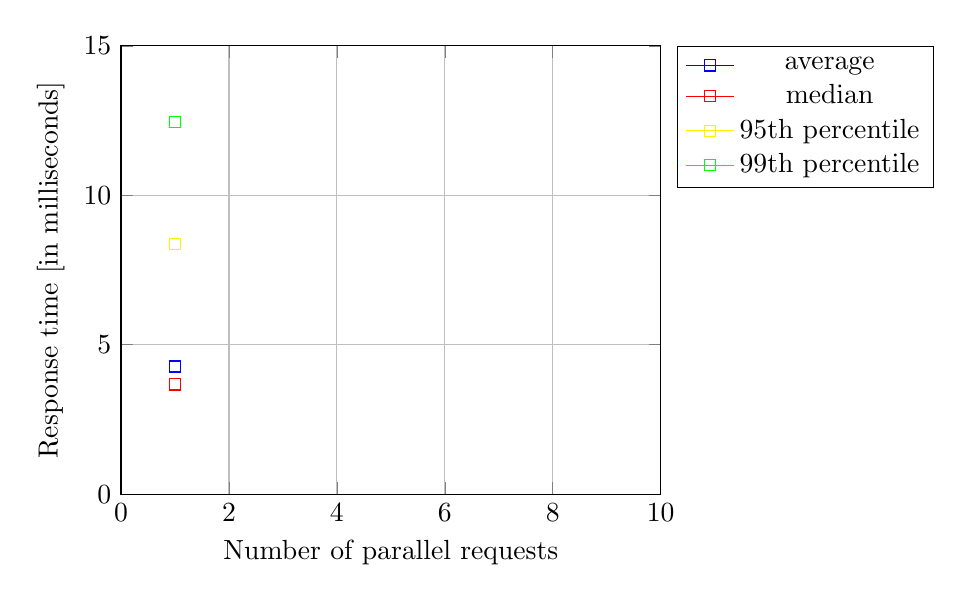
\begin{tikzpicture}[]
    \begin{axis}[
        xlabel={Number of parallel requests},
        ylabel={Response time [in milliseconds]},
        xmin=0, xmax=10,
        ymin=0, ymax=15,
        %legend pos=north west,
        grid=major,
        grid style=thin,
        legend pos=outer north east
      ]
        \addplot[
          color=blue,
          mark=square,
        ]
        coordinates {
          (1,   4.27)
        };
        \addlegendentry{average}

        \addplot[
          color=red,
          mark=square,
        ]
        coordinates {
          (1,   3.67)
        };
        \addlegendentry{median}

        \addplot[
          color=yellow,
          mark=square,
        ]
        coordinates {
          (1,   8.37)
        };
        \addlegendentry{95th percentile}

        \addplot[
          color=green,
          mark=square,
        ]
        coordinates {
          (1,   12.44)
        };
        \addlegendentry{99th percentile}
    \end{axis}
  \end{tikzpicture}
  \caption{Response time with query expansion}
  \label{fig:query-expansion}
\end{figure}
